\documentclass[a4paper]{article}

%% Language and font encodings
\usepackage[english]{babel}
\usepackage[utf8x]{inputenc}
\usepackage[T1]{fontenc}
\usepackage{subcaption}
\usepackage[parfill]{parskip}
\usepackage{url}
\def\UrlBreaks{\do\/\do-}
\usepackage{breakurl}

%% Sets page size and margins
\usepackage[a4paper,top=3cm,bottom=2cm,left=3cm,right=3cm,marginparwidth=1.75cm]{geometry}

%% Useful packages
\usepackage{amsmath}
\usepackage{graphicx}
\usepackage[colorinlistoftodos]{todonotes}
\usepackage[colorlinks=true, allcolors=blue, breaklinks]{hyperref}

\title{Symbols, Patterns, and Signals - Coursework Report}
\author{
  Rutterford, Ainsley\\
  \texttt{ar16478@my.bristol.ac.uk}
  \and
  Waugh, Harry\\
  \texttt{hw16471@my.bristol.ac.uk}
}

\begin{document}
\maketitle
\section{Introduction}

The aim of this assignment was to help students better understand, and gain experience in, clustering and classifying data. Why would it be useful to gain experience in these practices? Cluster analysis has a myriad of uses, such as outlier removal \cite{outlierremoval}, or image segmentation. There are many different techniques that are used for image segmentation, but the clustering method is one of the most efficient \cite{imagesegment}. In this report, we will explore the different methods used for clustering and data classification, focusing especially on nearest-centroid  classification and maximum-likelihood classification.

\section{Feature selection}

Each instance in our training data set was described by 5 feature vectors. We were asked to divide our data set of instances into subsets, such that each subset is associated with a class. It's worth noting that, although our task is to derive class labels for our data, if we had been provided with class labels for our data, there would be many methods one could use for feature selection, such as  forward feature selection, backward feature elimination, or recursive feature elimination \cite{featureselection}. However, since we are carrying out unsupervised learning, visually inspecting the data is adequate.

In order to visually assess which pair of features would best classify the data, we plotted every feature against each other in a scatterplot matrix. A scatter plot matrix contains all the pairwise scatter plots of the feature vectors in a matrix format \cite{scatterplot}. In order to ascertain the best features to identify the classes, we considered the following characteristics of each plot: the amount of clusters, the tightness of each cluster, and the number of outlying data points. 
\begin{figure}[h!]
\centering
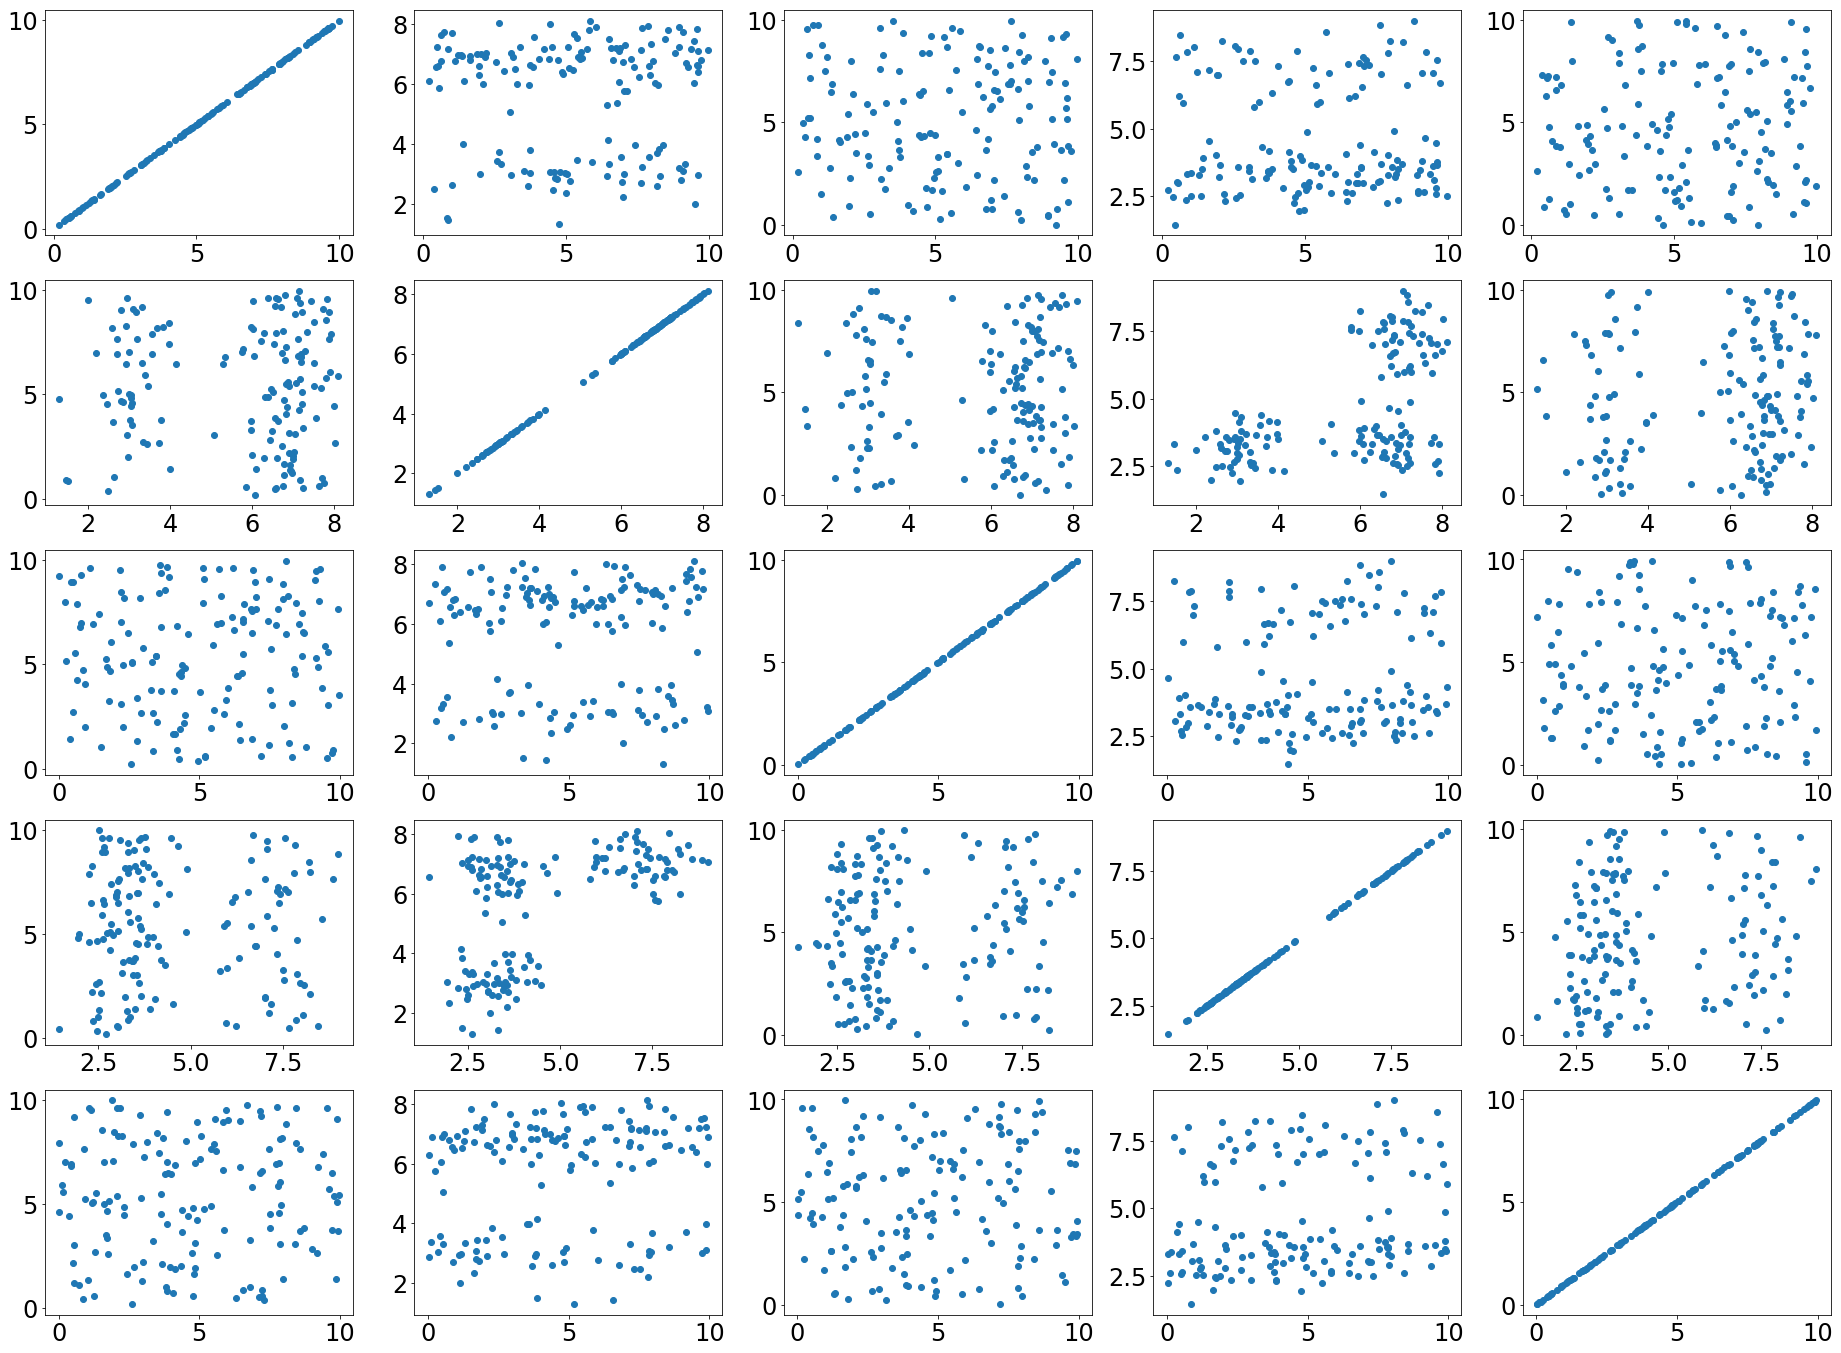
\includegraphics[width=1\columnwidth]{plot1.png}
\caption{Scatterplot matrix of the ar16478 training data set}
\end{figure}

After plotting the scatter plot matrix, we found that most feature pairs did not visually distinguish the classes adequately. Most features separated the data into two classes. The one exception to this was the plotting of features 2 and 4. This plot yielded 3 very easily distinguishable clusters that were compact and contained most of the data. After identifying the features that best separated the data, we assembled a matrix with 2 columns containing only these two feature vectors to use for the remainder of the assignment.

\section{Identifying the classes}

Since we are carrying out unsupervised learning (as our data set is 'unlabeled'), we then needed to derive class labels for each of the data points in our training data set. The model produced could then be used to classify any future test data. We achieved this though cluster analyses, or clustering. So what is clustering? Clustering is the task of dividing data points into K groups such that the data points in each group are more similar to each other than to the data points in other groups \cite{clusteringdef}. There are many centroid based clustering algorithms one could choose from, such as K-Medoids or Fuzzy C-Means, all with varying characteristics, such as sensitivity to outliers or time complexity \cite{clarion}, but ultimately we chose the K-Means algorithm to cluster our data.

The aim of the K-Means algorithm is to divide M points in N dimensions into K clusters so that the within-cluster sum of squares is minimized \cite{kmeans}. Initially, K-Means chooses K points to be the initial cluster centers. The methods used to select these initial points vary; this will be relevant later on. K-Means then assigns every data point a cluster,  choosing whichever cluster center has the minimum euclidean distance from the data point. After this, the cluster centers are recalculated based on the mean position of its current data points. Again, all the data is assigned a cluster. K-Means iterates through these steps until the cluster centers no longer change after an iteration. At this point some kind of an optimal data clustering has then been found \cite{clarion}. Note that it may not necessarily be a global optimum, but we will explore this further in the next section.

We applied the K-Means clustering algorithm to our training data set to obtain the class labels for each data point and the cluster center points. The latter will be used for our nearest-centroid classification later on. Using the class labels, we split the data set into 3 classes. We noticed that the classes were of equal size, which again will be important later on.

\section{Nearest-centroid classification}

We were now able to use the centroids provided by K-Means as a nearest-centroid classifier. The next task was to use this classifier to classify instances from a test data set we were provided with. For each data point, the cluster center with the minimum euclidean distance from the data point was selected. The data point was then part of the class associated with the selected cluster center.  We classified the test data, and plotted the test and training data alongside a voronoi diagram, shown in Figure 2.


\begin{figure}[h!]
\centering
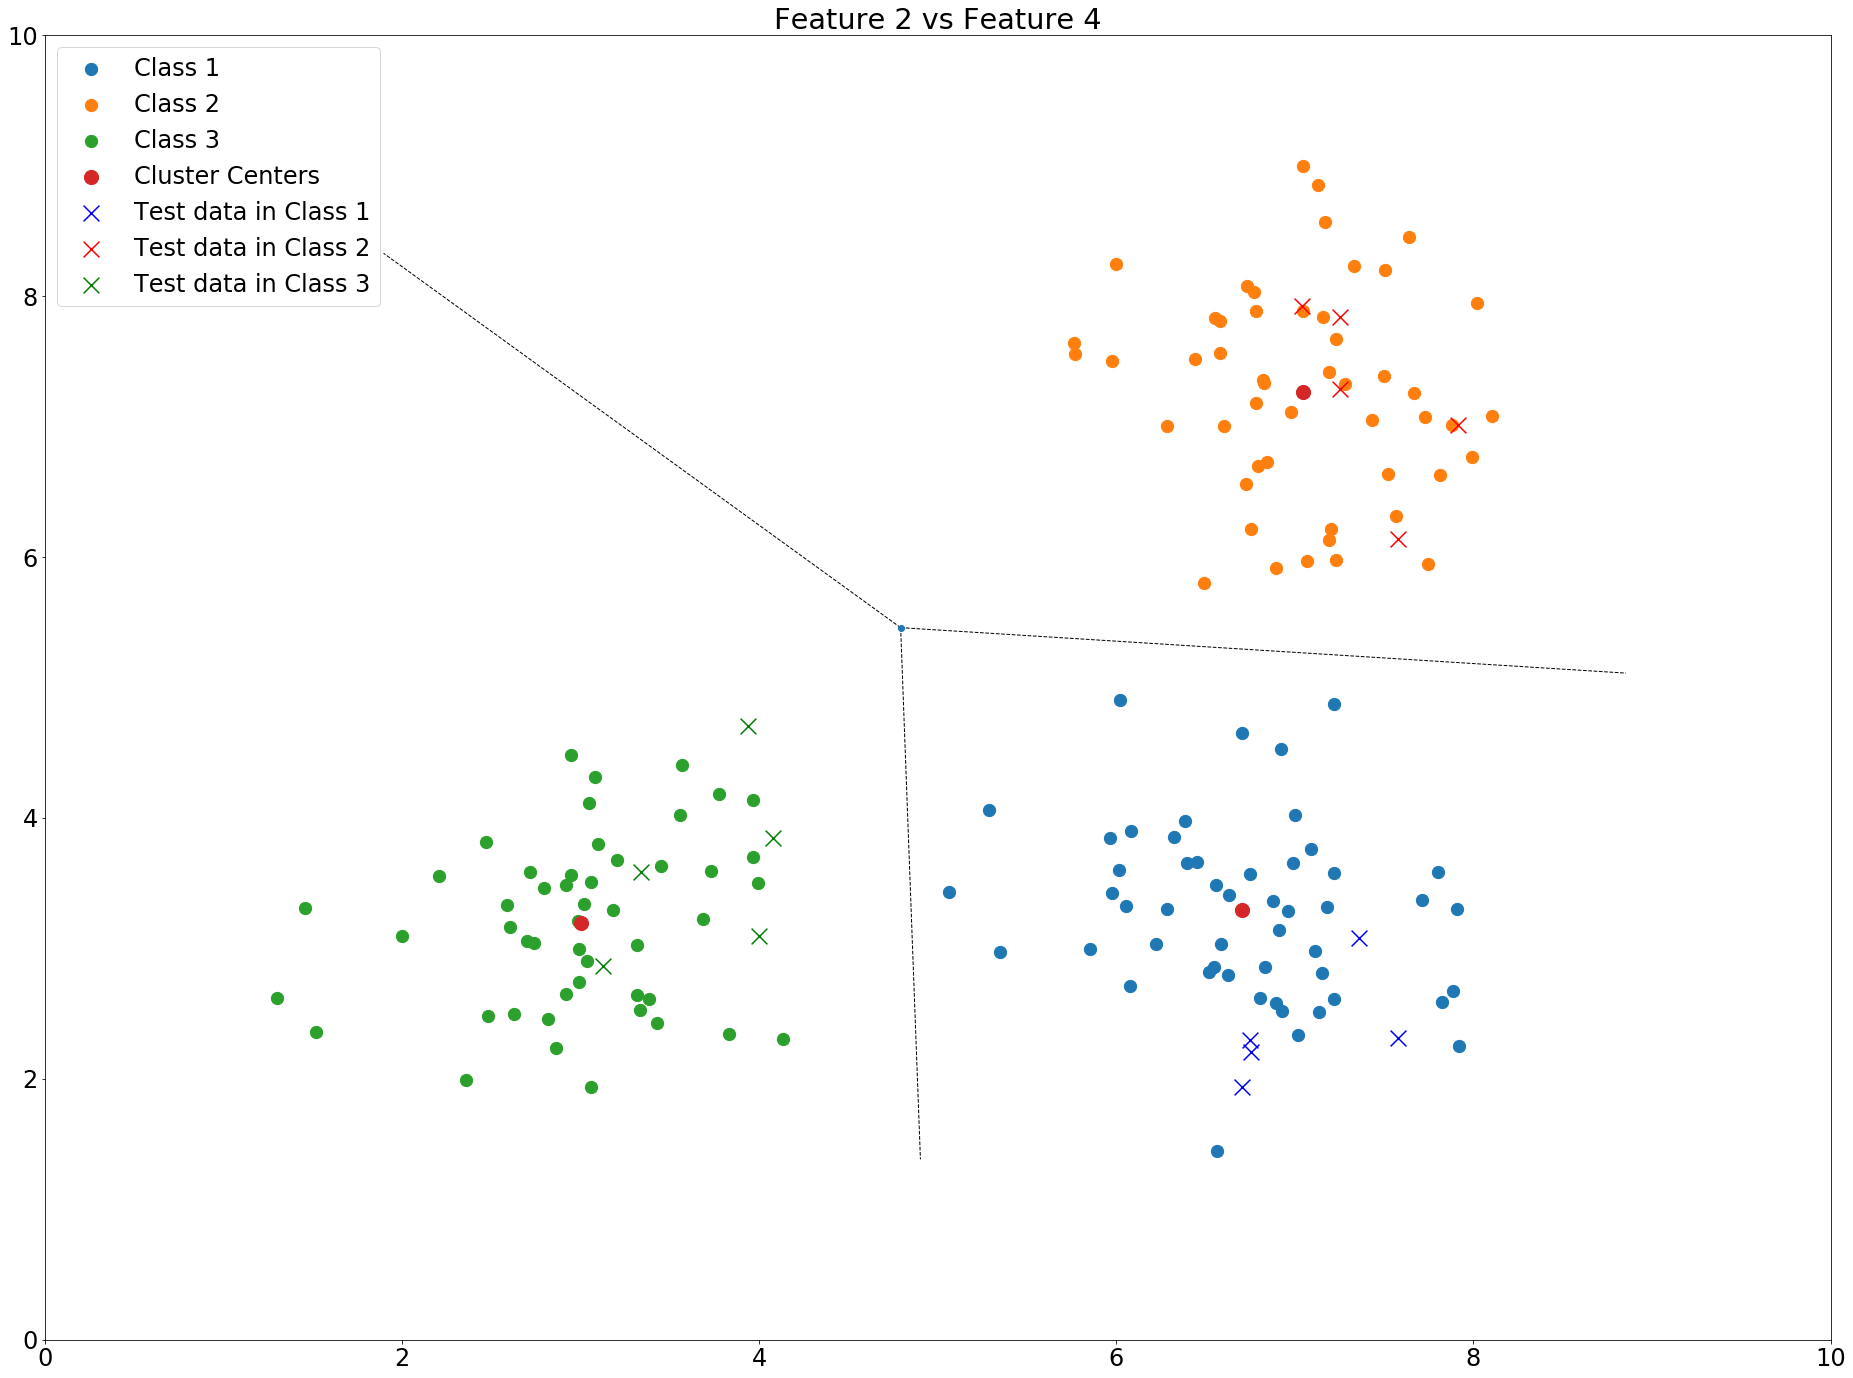
\includegraphics[width=1\columnwidth]{plot2.png}
\caption{Plotting the 3 classes with a voronoi plot}
\end{figure}

We were then asked to find a deliberately non-optimal clustering by manipulating the K-means algorithm in some way. There are many ways one could go about achieving this. Originally, we were supplying the K-Means algorithm with non-optimal starting points and limiting the number of iterations that K-Means could complete. This did produce a non optimal clustering, but this was not a fair solution for multiple reasons. Firstly, this approach required some kind of prior knowledge of the cluster centers' positions, which would not always be available. Secondly, K-Means is not guaranteed to return a globally optimum clustering, but it is guaranteed to return a local optimum \cite{kmeans}, and is guaranteed to terminate given enough iterations \cite{kmeansintro}. We were not allowing K-Means to terminate at all and so we did not allow the algorithm to actually find a local optimum. 

Put simply, our second approach was to run the K-Means algorithm many times, and to plot the run that terminated at the worst clustering found. With our second approach, we allowed the algorithm to complete the default amount of iterations to ensure a local optimum was indeed found. However, as mentioned earlier, the methods for choosing the initial cluster center points can vary. By default, K-Means was using an initialisation method called 'K-Means\texttt{+}\texttt{+}', which enabled the algorithm to choose a much better initial set of cluster centers. We changed the initialisation method to 'random' which meant that the initial cluster centers were any random set of points \cite{scikit-learn}. This is important as using 'K-Means\texttt{+}\texttt{+}' would mean that finding a non optimal clustering would require a great deal of runs.

Another initialisation parameter we changed was the number of times the algorithm could run with different initial centroid points. We limited this to 1. Any higher number than this would again require a vast amount of runs in order to find a non optimal clustering. With these new initialisation parameters, we ran K-Means 1000 times and took the run which produced the highest inertia. Inertia is the squared sum of the distances between each point and its closest cluster center. So, by selecting the run with the greatest inertia, we would be selecting the run with the least optimal clustering.

\begin{figure}[h!]
\centering
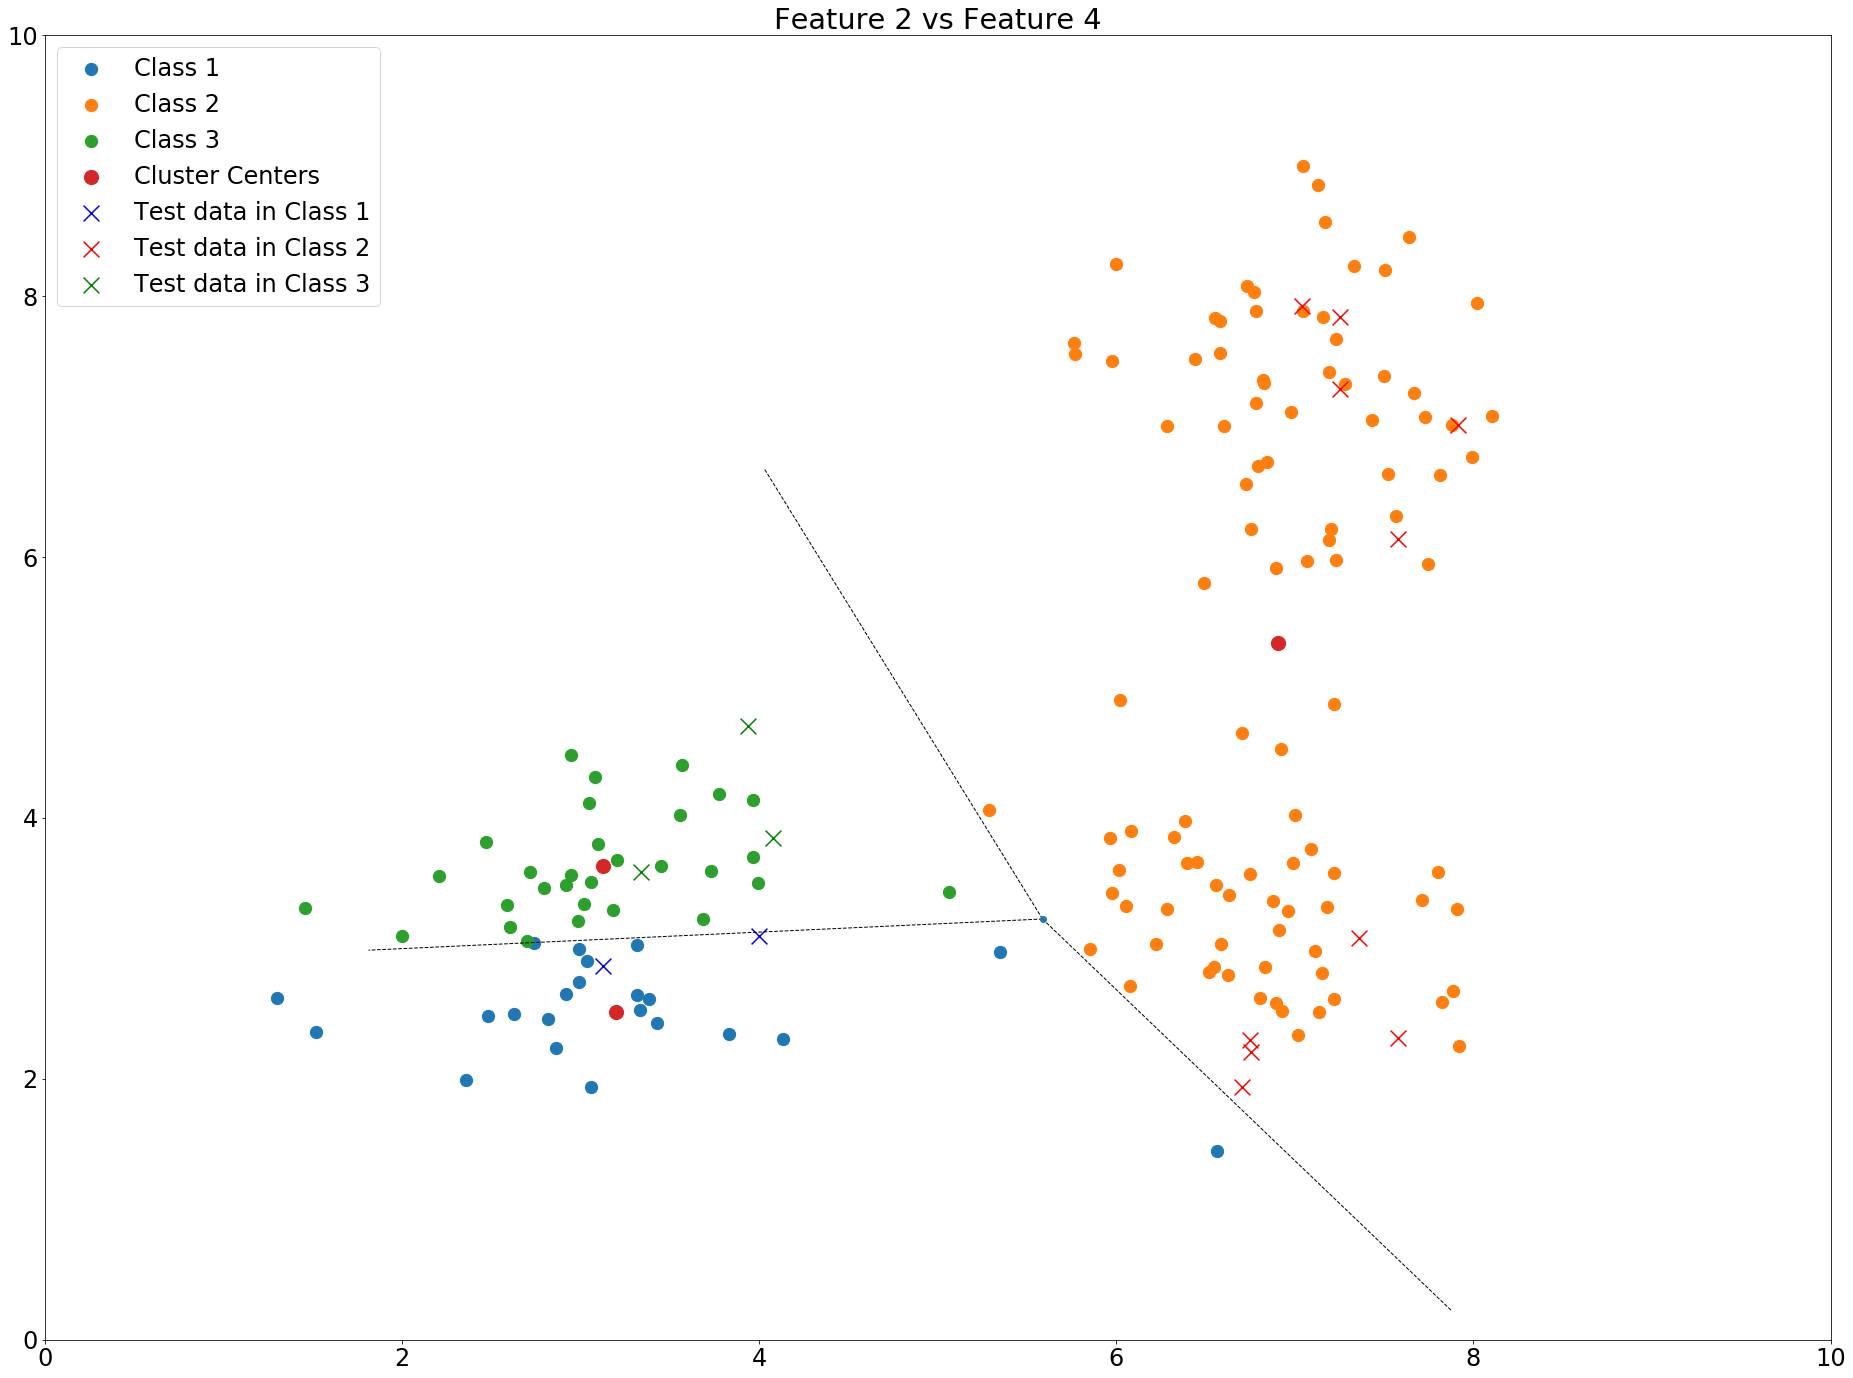
\includegraphics[width=1\columnwidth]{plot3.png}
\caption{Plotting a deliberately non optimal clustering with the updated classes and voronoi plot}
\end{figure}

\section{Maximum-likelihood classification}

The first step to creating a maximum likelihood classifier using our training data was to calculate the covariance matrices and means for each cluster. We then generated a matrix containing the coordinates of 40,000 evenly spaced points spanning our entire graph. For each of these points we calculated the Mahalanobis distance to each of the clusters. The Mahalanobis distance is a multi-variate method of calculating the distance between a point P and its distribution D \cite{mahalwiki}, in other words, it is the number of standard deviations between P and D. If the axes were changed to increment in units equal to the variance, the Mahalanobis distance would be simply the Euclidean distance between P and the D's mean. In order to calculate the Mahalanobis distance we used the following formula:
\begin{equation}
(x - u)^T \ \Sigma ^ {-1} \ (x - u) 
\end{equation}
Where $x$ is the data point, $u$ is the mean of a cluster, and $\Sigma$ is the covariance matrix of the cluster. We then plotted each clusters' contour along all the points where the Mahalanobis distance to that cluster was equal to 5.9915. This figure was calculated using the inverse of the chi distribution \cite{chidist}. This translates a given number of degrees of freedom and threshold probability for each cluster, to the Mahalanobis distance. In our data we used a threshold of 0.95, meaning we wanted the contour to contain 95\% of the data, along with 2 degrees of freedom, due to our bivariate distribution.

We were then asked to plot decision boundaries between each pair of classes, in order to plot these we looked at what the decision boundary actually represents with regards to clustering the data. We realised that it was a line of all the points that were equidistant from both cluster centers. Therefore to determine the decision boundaries for our maximum-likelihood classifier, we would be checking each point in the space for an equal Mahalanobis distance to both clusters, or the ratio of these distances being 1:1. 

We could then manipulate this information to create more complex decision boundaries, for example if we knew previously that class A was twice as likely as class B, we could incorporate this prior probability by looking for all the points that had a distance ratio of cluster A to B of 2:1. As all of the data given to us made up 3 equal classes of size 50, we didn't have to worry about incorporating a prior probability as every data point had an equal chance of being in each class.

Another way we could manipulate the maximum-likelihood classifier decision boundaries, is to make them resemble the ones shown by the Voronoi diagram in Figure 2. Recall that in order to calculate the Mahalanobis distance from a point to a cluster, we had to consider a clusters' covariance matrix to transform the axes into unit variance. However to generate a simple nearest centroid boundary we only need to pass in the identity matrix, this works because it effectively sets the the variance of both the features to 1 and the correlation between to 0. Hence, the Mahalanobis distance for each point becomes equal to the Euclidean distance to the clusters center, as the standard deviation for each cluster is now 1. This can be seen clearly when comparing Mahalanobis distance $D_M$ to Euclidean distance $D_E$ \cite{mahal}:
\begin{equation}
D_M = \sqrt[]{(x - u)^T \ \Sigma ^ {-1} \ (x - u)}
\end{equation}
\begin{equation}
D_E = \sqrt[]{(x - y)^T  \ (x - y)} 
\end{equation}
From the equations above we can now see that substituting the identity matrix for the covariance results in the Mahalanobis distance becoming equal to the Euclidean distance. 


\begin{figure}
\begin{subfigure}[h]{0.5\columnwidth}
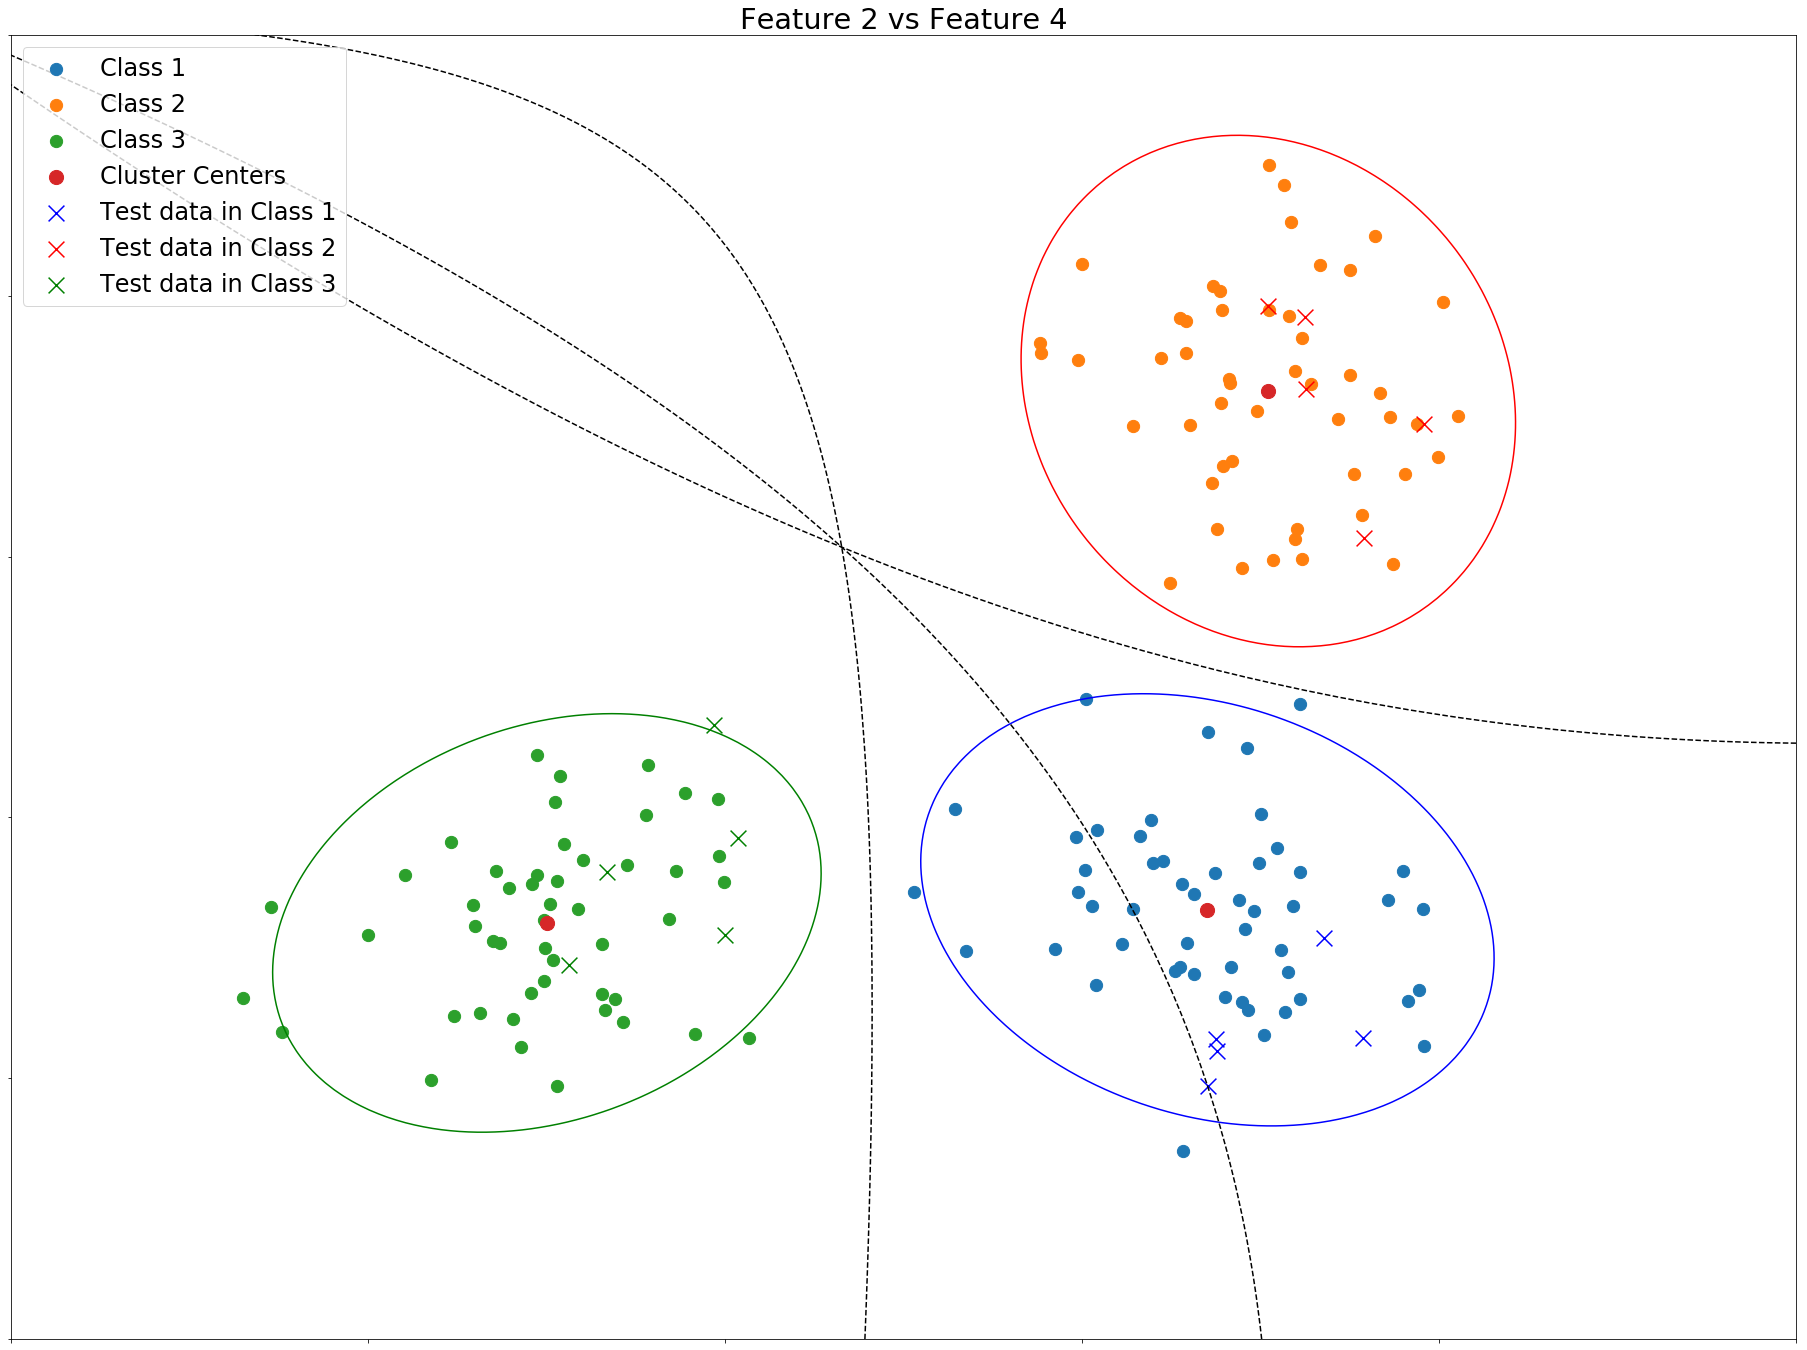
\includegraphics[width=\columnwidth]{plot4.png}
\end{subfigure}
\hfill
\begin{subfigure}[h]{0.5\columnwidth}
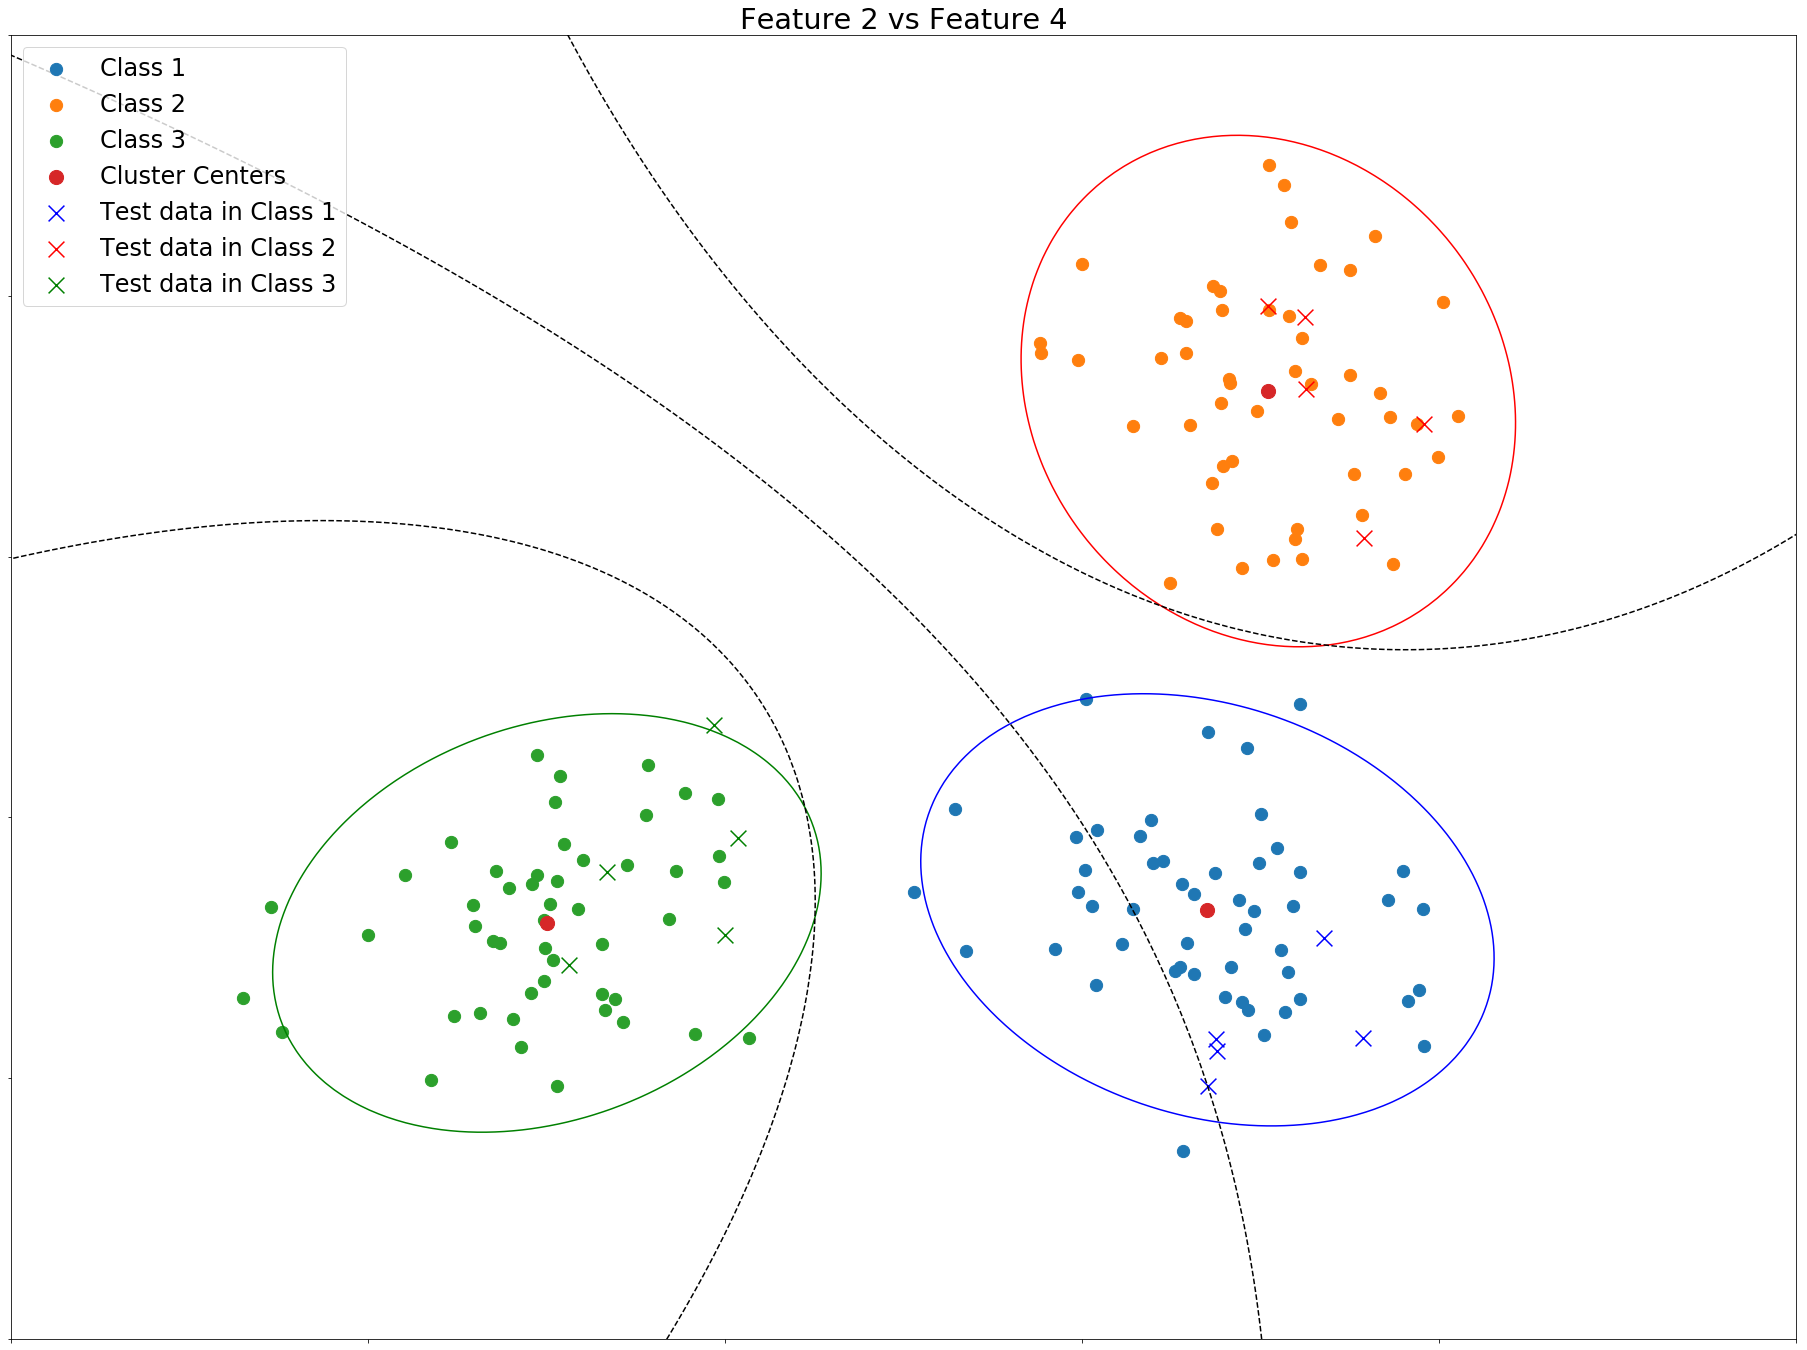
\includegraphics[width=\columnwidth]{plot5.png}
\end{subfigure}%
\caption{Comparing the decision boundaries when all classes are equally as likely (left), to the decision boundaries when class 1 is twice as likely as the others (right)}
\end{figure}

\section{Discussion of results}

When comparing the classifiers produced from the ar16478 training data set and the hw16471 training data set, we noticed that there were no discrepancies between the nearest-centroid and maximum-likelihood classified points in the ar16478 model. However, the hw16471 model contains 2 test data points that were classified differently by each classifier.

We also noticed that there is a point that belongs to a class in the nearest-centroid classifier, but when using maximum-likelihood to improve this classifier, this point now resided on the other side of the decision boundary. This is perfectly acceptable as the decision boundary only represents where two classes are equally as likely, so a point can be on one side of this boundary and still belong to a class on the other side of the boundary. If we were to try to manipulate the decision boundaries to account for this point, we would risk overfitting.

When plotting the ellipses that contained 95\% of the probability mass, we found that the hw16471 training data set had exactly 96\% of the points lying within the ellipses and the ar16478 training data set had 95.3\%. This small degree of error in the percentages are expected, as the theoretical probability suggests that the ellipses contain 95\% of the data points. If we were to have an infinitely large training data set, exactly 95\% of the points would lie within the ellipses. 

\begin{figure}
\begin{subfigure}[h]{0.5\columnwidth}
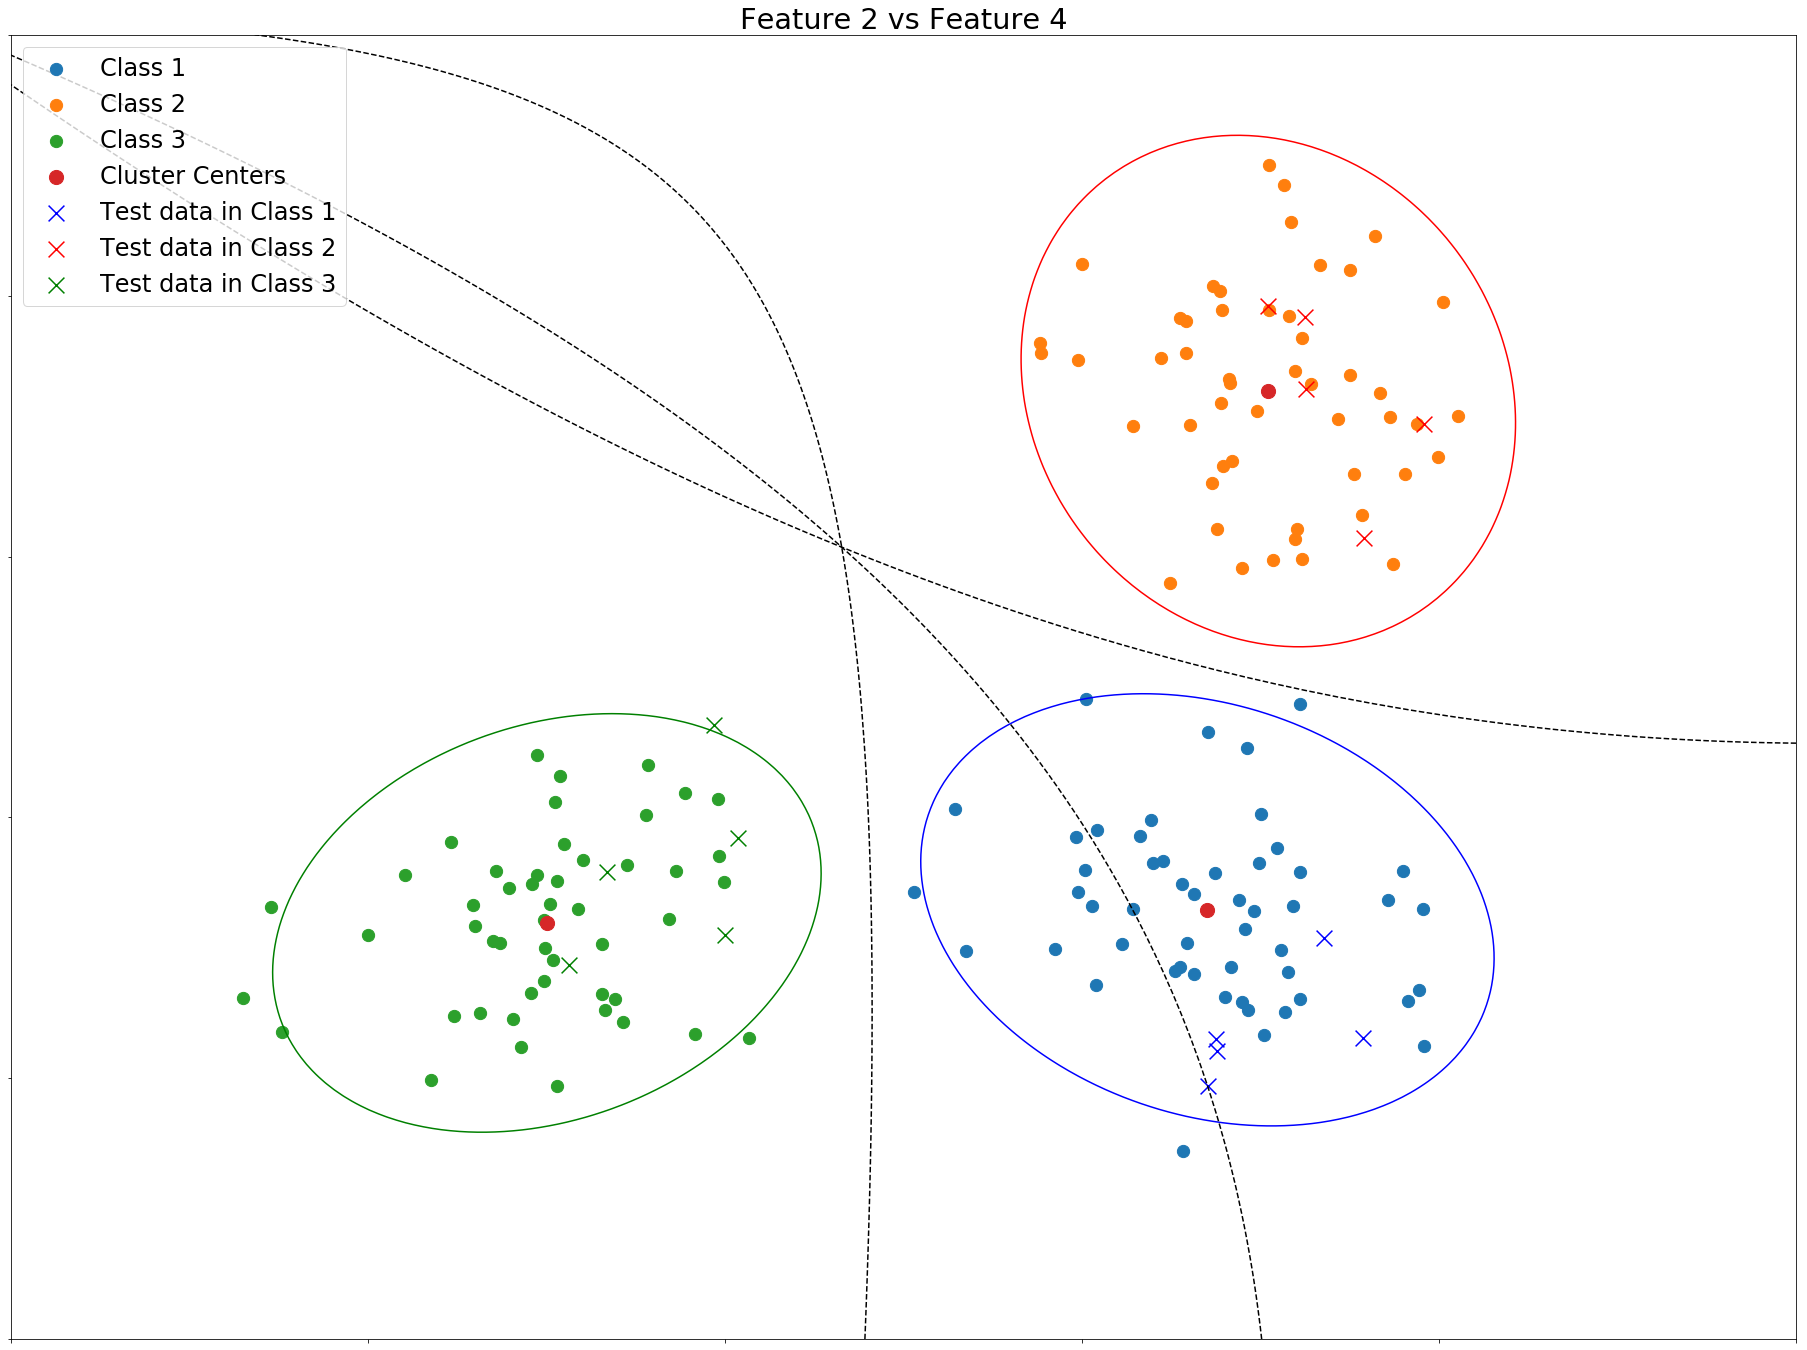
\includegraphics[width=\columnwidth]{plot4.png}
\end{subfigure}
\hfill
\begin{subfigure}[h]{0.5\columnwidth}
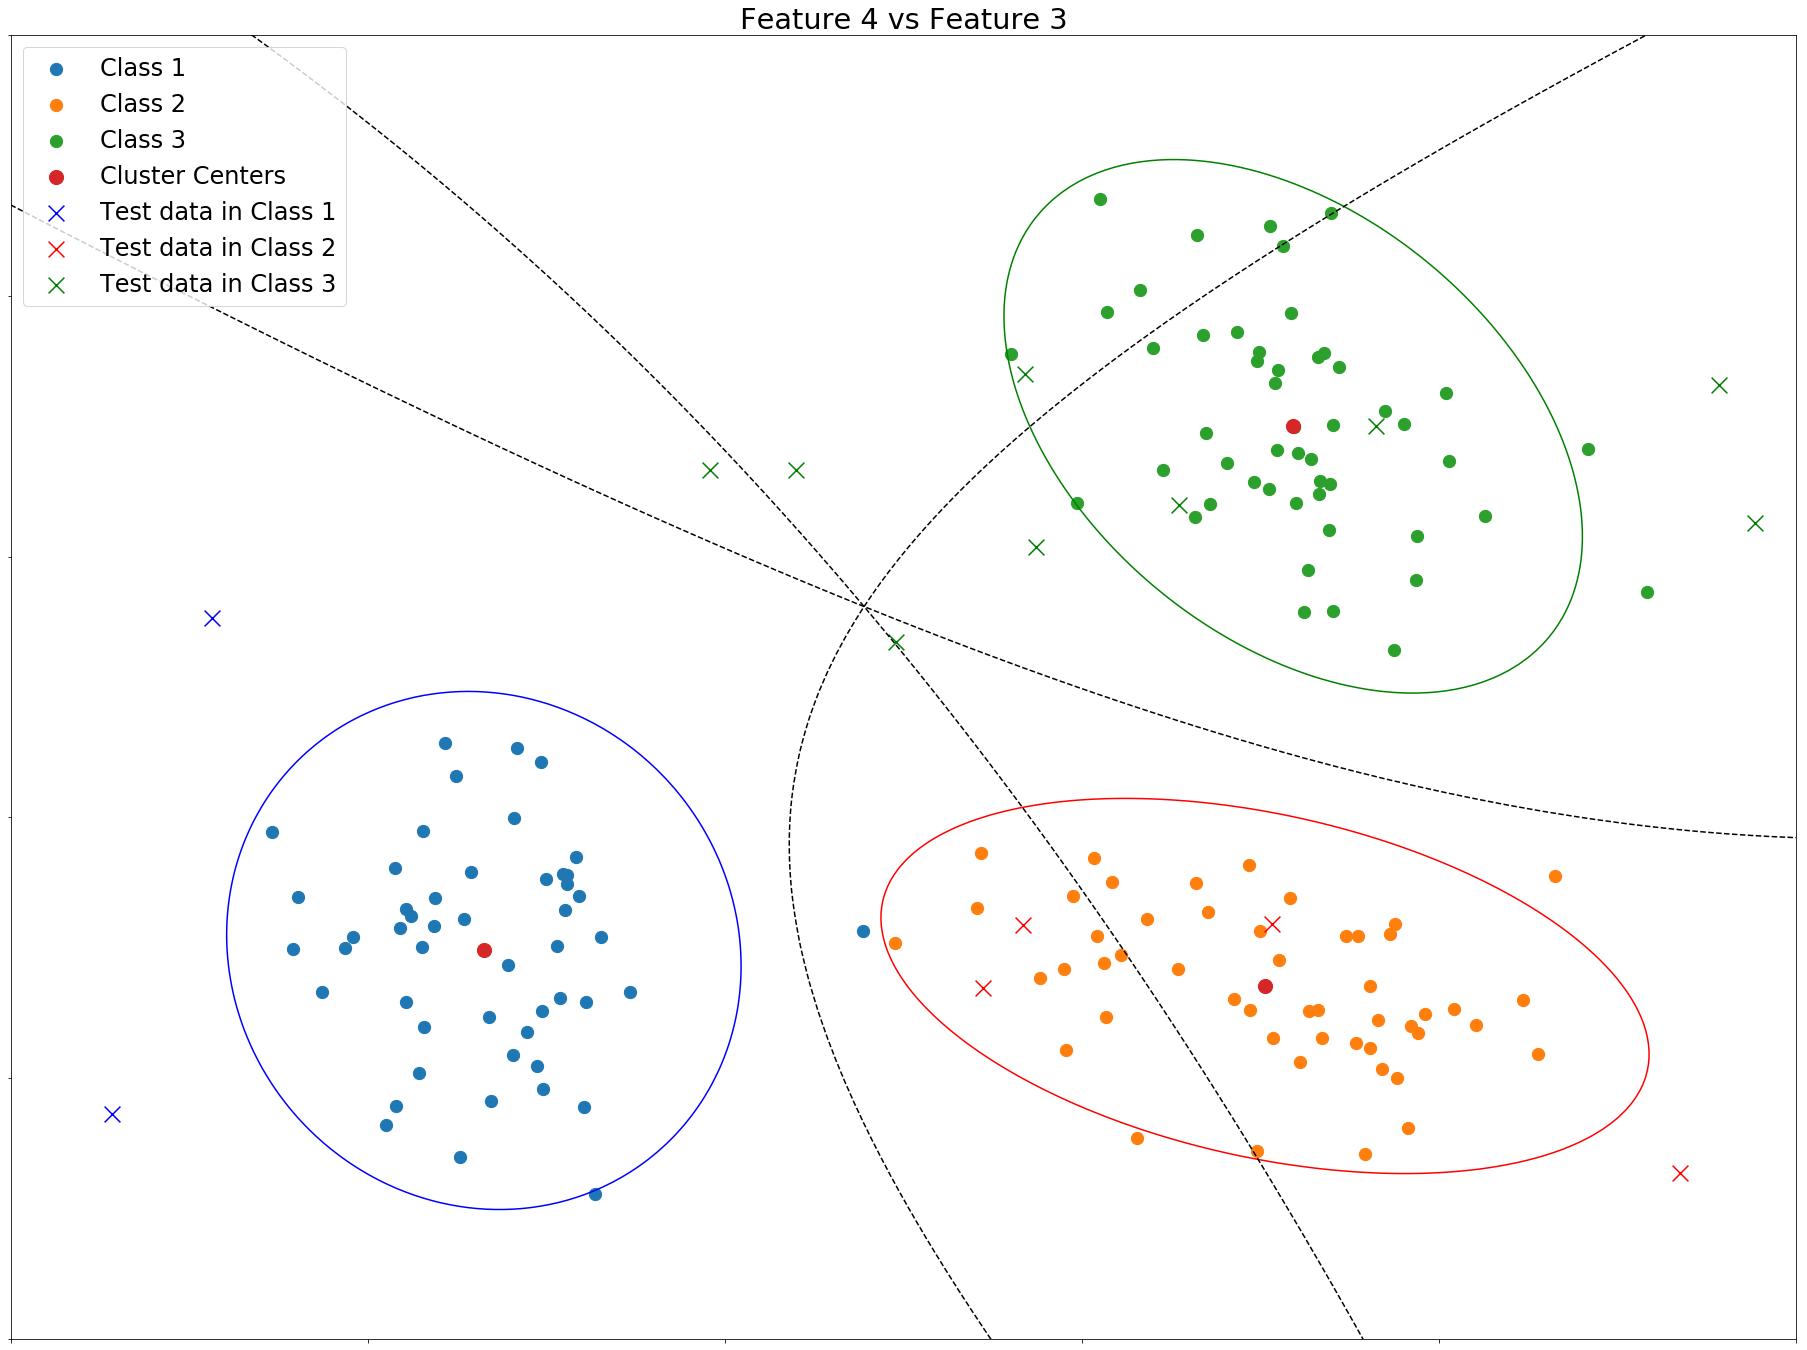
\includegraphics[width=\columnwidth]{plot6.png}
\end{subfigure}%
\caption{Comparing the ar16478 data sets (left) to the hw16471 data sets (right)}
\end{figure}

\bibliographystyle{abbrv}
\bibliography{sample}

\end{document}